\documentclass{article}
\usepackage{graphicx} % Required for inserting images
\usepackage{geometry}
\usepackage{textcomp}
\usepackage{amsmath}

\title{\textbf{MATH 209: HW 4}}
\author{Jeffery Zhang}
\date{Due: December 6th, 2023}
\begin{document}
\maketitle

\section{Question 1}
Solve the Laplace Equation on the unit square with Dirichlet Boundary conditions in the following cases:
\begin{center}
    \(\Delta u(x, y) = 0, \,\, u(x, 1) = f(x), \,\, u(x, 0) = u(0, y) = u(1, y) = 0\).
\end{center}
\begin{itemize}
    \item \(f(x) = 3\sin (3\pi x) - 2\sin(\pi x)\)
    \item \(f(x) = 1\)
\end{itemize}
Since the function is only at \(y = 1\), the generalized equations are as follows:
\begin{center}
    \(\displaystyle u(x, y) = \sum_{n = 0}^{\infty}c_n\sin(n\pi x)\sinh(n\pi y)\)\\*[10pt]
    \(\displaystyle c_n = \frac{2\int_{0}^{1}f(x)\sin (n\pi x)dx}{\sinh(\pi n)}\)
\end{center}
\rule{\linewidth}{0.2mm}\\*[10pt]
\textbf{a.)} Since \(f(x)\) is in the form \(c_n\sin(n\pi x)\), we have to find the coefficients \(c_1\) and \(c_3\) that satisfy the equation:
\begin{center}
    \(\displaystyle u(x, 1) = \sum_{n = 0}^{\infty}c_n\sin(n\pi x)\sinh(n\pi) = 3\sin (3\pi x) - 2\sin(\pi x)\)\\*[10pt]
    \(\displaystyle c_1\sinh(\pi)\sin(\pi x) = -2\sin(\pi x)\rightarrow c_1 = -\frac{2}{\sinh(\pi)}\)\\*[10pt]
    Likewise, \(\displaystyle c_3 = \frac{3}{\sinh(3\pi)}\)
\end{center}
Therefore, the fully generalized solution is:
\begin{center}
    \boxed {
        \(\displaystyle u(x, y) = \frac{3}{\sinh(3\pi)}\sin(3\pi x)\sinh(3\pi y) - \frac{2}{\sinh(\pi)}\sin(\pi x)\sinh(\pi y)\)
    }
\end{center}
\textbf{b.)} \(\displaystyle c_n = \frac{2\int_{0}^{1}\sin (n\pi x)dx}{\sinh(\pi n)}\rightarrow \frac{2 - 2\cos (\pi n)}{\pi n\sinh(\pi n)}\), which is 0 if n is even, and \(\displaystyle\frac{4}{\pi n\sinh(\pi n)}\) otherwise. \\*[10pt]
Therefore, the fully generalized solution is:
\begin{center}
    \boxed {
        \(\displaystyle u(x, y) = \sum_{n \, = \, odd}^{\infty}\frac{4\sin(n\pi x)\sinh(n\pi y)}{\pi n\sinh(\pi n)}\)
    }
\end{center}

\clearpage \noindent
\section{Question 2}
Solve the Laplace equation on the circle of \(r = 1\) with Dirichlet boundary conditions in the following cases:
\begin{center}
    \(\Delta u(r, \theta) = 0, \,\, u(1, \theta) = f(\theta), \,\, \theta \in [-\pi, \pi)\)
\end{center}
\begin{itemize}
    \item \(f(\theta) = 1 + \cos (\theta) - \sin(2\theta)\)
    \item \(f(\theta) = 0\) if \(\theta \in [-\pi, 0), \,\, f(\theta) = 1\) if \(\theta \in [0, \pi)\)
    \item \(f(\theta) = 3\theta + 2\theta^{17} - \sin^3(\theta)\) for \(r = 0\)
\end{itemize}
Since \(r = 1\), the generalized equations are as follows:
\begin{center}
    \(\displaystyle u(r, \theta) = a_0 + \sum_{n = 1}^{\infty}(a_n\cos(n\theta) + b_n\sin(n\theta))r^n\)\\*[10pt]
    \(\displaystyle a_n = \frac{1}{\pi}\int_{-\pi}^{\pi}f(\theta)\cos(n\theta)d\theta\)\\*[10pt]
    \(\displaystyle b_n = \frac{1}{\pi}\int_{-\pi}^{\pi}f(\theta)\sin(n\theta)d\theta\)\\*[10pt]
    \(\displaystyle a_0 = \frac{1}{2\pi}\int_{-\pi}^{\pi}f(\theta)d\theta\)
\end{center}
\rule{\linewidth}{0.2mm}\\*[10pt]
\textbf{a.)} Applying the same method as Question 1, we have to solve for \(a_1\) and \(b_2\). But first, we have to evaluate for \(a_0\) for all terms. It turns out that \(a_0 = 1\) for only the 1 term, and \(a_0 = 0\) for the rest. So then, \(a_1\) and \(b_2\) are also both 1. Integrating for the 1 term, we get:
\begin{center}
    \(\displaystyle a_n = \frac{1}{\pi}\int_{-\pi}^{\pi}\cos(n\theta)d\theta\rightarrow\) 0 for all n.\\*[10pt]
    \(\displaystyle b_n = \frac{1}{\pi}\int_{-\pi}^{\pi}\sin(n\theta)d\theta\rightarrow\) 0 because of odd function.
\end{center}
Therefore, the fully generalized function is:
\begin{center}
    \boxed{
        \(u(r, \theta) = 1 + r\cos(\theta) - r^2\sin(2\theta)\)
    }
\end{center}
\textbf{b.)} The integrals go as follows:
\begin{center}
    \(\displaystyle a_n = \frac{1}{\pi}\int_{0}^{\pi}\cos(n\theta)d\theta\rightarrow\) 0 for all n.\\*[10pt]
    \(\displaystyle b_n = \frac{1}{\pi}\int_{0}^{\pi}\sin(n\theta)d\theta\rightarrow\frac{1 - \cos(\pi n)}{\pi n}\rightarrow\) 0 for all even n, \(\displaystyle\frac{2}{\pi n}\) otherwise.\\*[10pt]
    \(\displaystyle a_0 = \frac{1}{2\pi}\int_{0}^{\pi}d\theta\rightarrow \frac{1}{2}\)
\end{center}
Therefore, the fully generalized solution is as follows:
\begin{center}
    \boxed{
        \(\displaystyle u(r, \theta) = \frac{1}{2} + \sum_{n = odd}^{\infty}\frac{2\sin(n\theta)r^n}{\pi n}\)
    }
\end{center}
\textbf{c.)} Since \(r = 0\), the whole summation section of the generalized solution goes to 0. Therefore, we only worry about \(a_0\). However, since \(f(\theta)\) is odd, \(a_0\) is also 0. Therefore, \(u(r, \theta) = 0\) at \(r = 0\).

\clearpage \noindent
\section{Question 3}
Plot the solution of the wave equation on the line \(x\in (-\infty , \infty)\)
\begin{center}
    \(\displaystyle \frac{\partial^2u}{\partial t^2}(t, x) = \frac{\partial^2u}{\partial x^2}(t, x), \,\, u(0, x) = f(x), \,\, \frac{\partial u}{\partial t}(0, x) = g(x)\)
\end{center}
for values of time \(t = 0, \,\, t = 1/2, \,\, t = 1, \,\, t = 3/2,\) and \(t = 2\) in the following cases:
\begin{itemize}
    \item \(\displaystyle f(x) = \frac{1}{1+x^2}, \,\, g(x) = 0\)
    \item \(f(x) = 1\) if \(x \in [1/2, \, 3/2], \,\, f(x) = -1\) if \(x\in [-3/2, \, -1/2], \,\, f(x) = 0\) otherwise, and \(g(x) = 0\)
    \item \(f(x) = 0\) and \(g(x) = 1\) if \(x\in [-1, 1]\), \, \(g(x) = 0\) otherwise. \\
\end{itemize}
The generalized D'Alembert solution is as follows:
\begin{center}
    \(\displaystyle u(t, x) = \frac{f(x - t) + f(x + t)}{2} + \frac{1}{2}\int_{x - t}^{x + t}g(x)dx\)
\end{center}
\rule{\linewidth}{0.2mm}\\*[10pt]
\textbf{a.)} Plugging in \(\displaystyle\frac{1}{1 + x^2}\) into \(\displaystyle\frac{f(x - t) + f(x + t)}{2}\), we get the expression:
\begin{center}
    \(\displaystyle u(x, t) = \frac{1}{2 + 2(x - t)^2} + \frac{1}{2 + 2(x + t)^2}\)\\*[10pt]
\end{center}
Sketches of this function are on the last page. \\*[10pt]
\textbf{b.)} Following intuitively from the last problem, the initial profile "splits in half" and starts propagating both to the left and to the right, leading to various constructive and destructive interferences. Sketches of this function are on the last page. \\*[10pt]
\textbf{c.)} If we imagine \(u(t, x)\) as a surface, we know that the derivative in the "t" direction is initially 1 between \([-1, 1]\). Therefore, it will look like a growing triangle (with slopes 1/2, due to the 1/2 factor in front of the integral). Such a triangle can only grow vertically up to 1, due to the initial condition (if the initial condition was \(g(x) = 1\) if \(x\in [-2, 2]\), for example, the triangle would vertically grow to 2 instead). After this, each side propagates away from the origin at 1 unit per unit time. Sketches of this function are on the last page. 

\clearpage \noindent
\begin{figure}
    \centering
    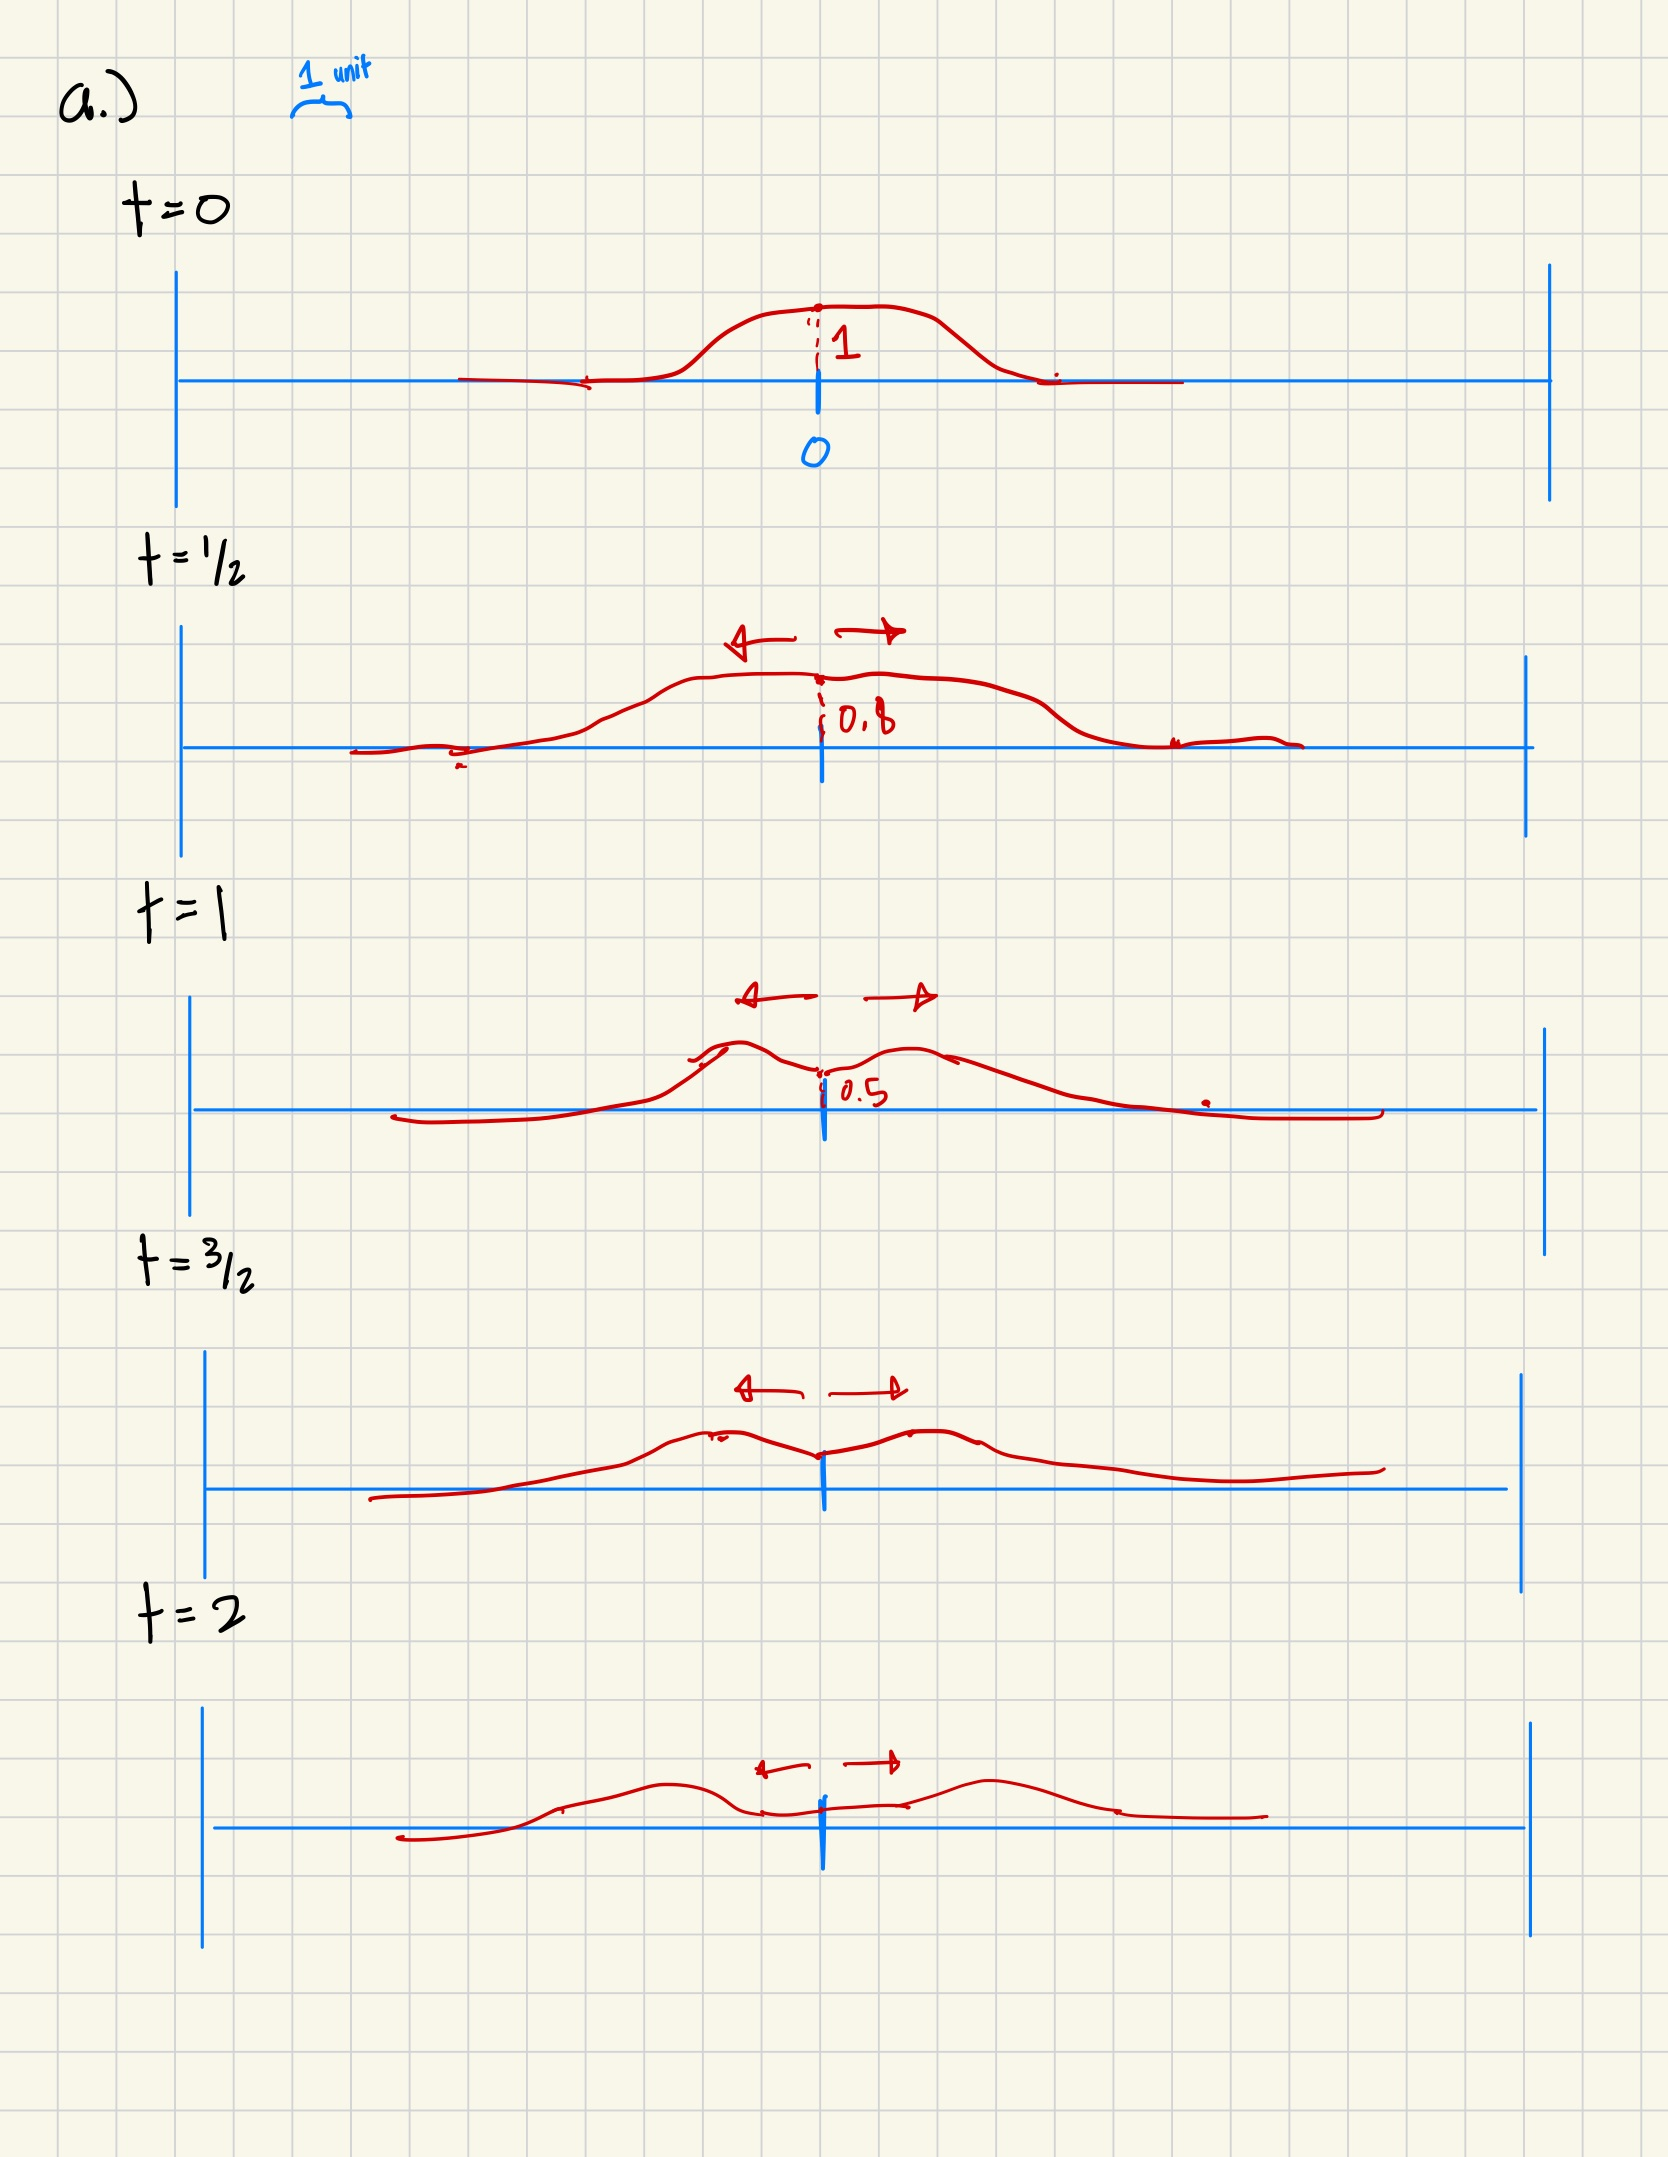
\includegraphics[width=0.4\textwidth]{HW_4_Plots-a.jpg}
    \caption{Sketch for Problem 3a. Note: 1 square/unit}
    \label{fig:sample}
\end{figure}
\begin{figure}
    \centering
    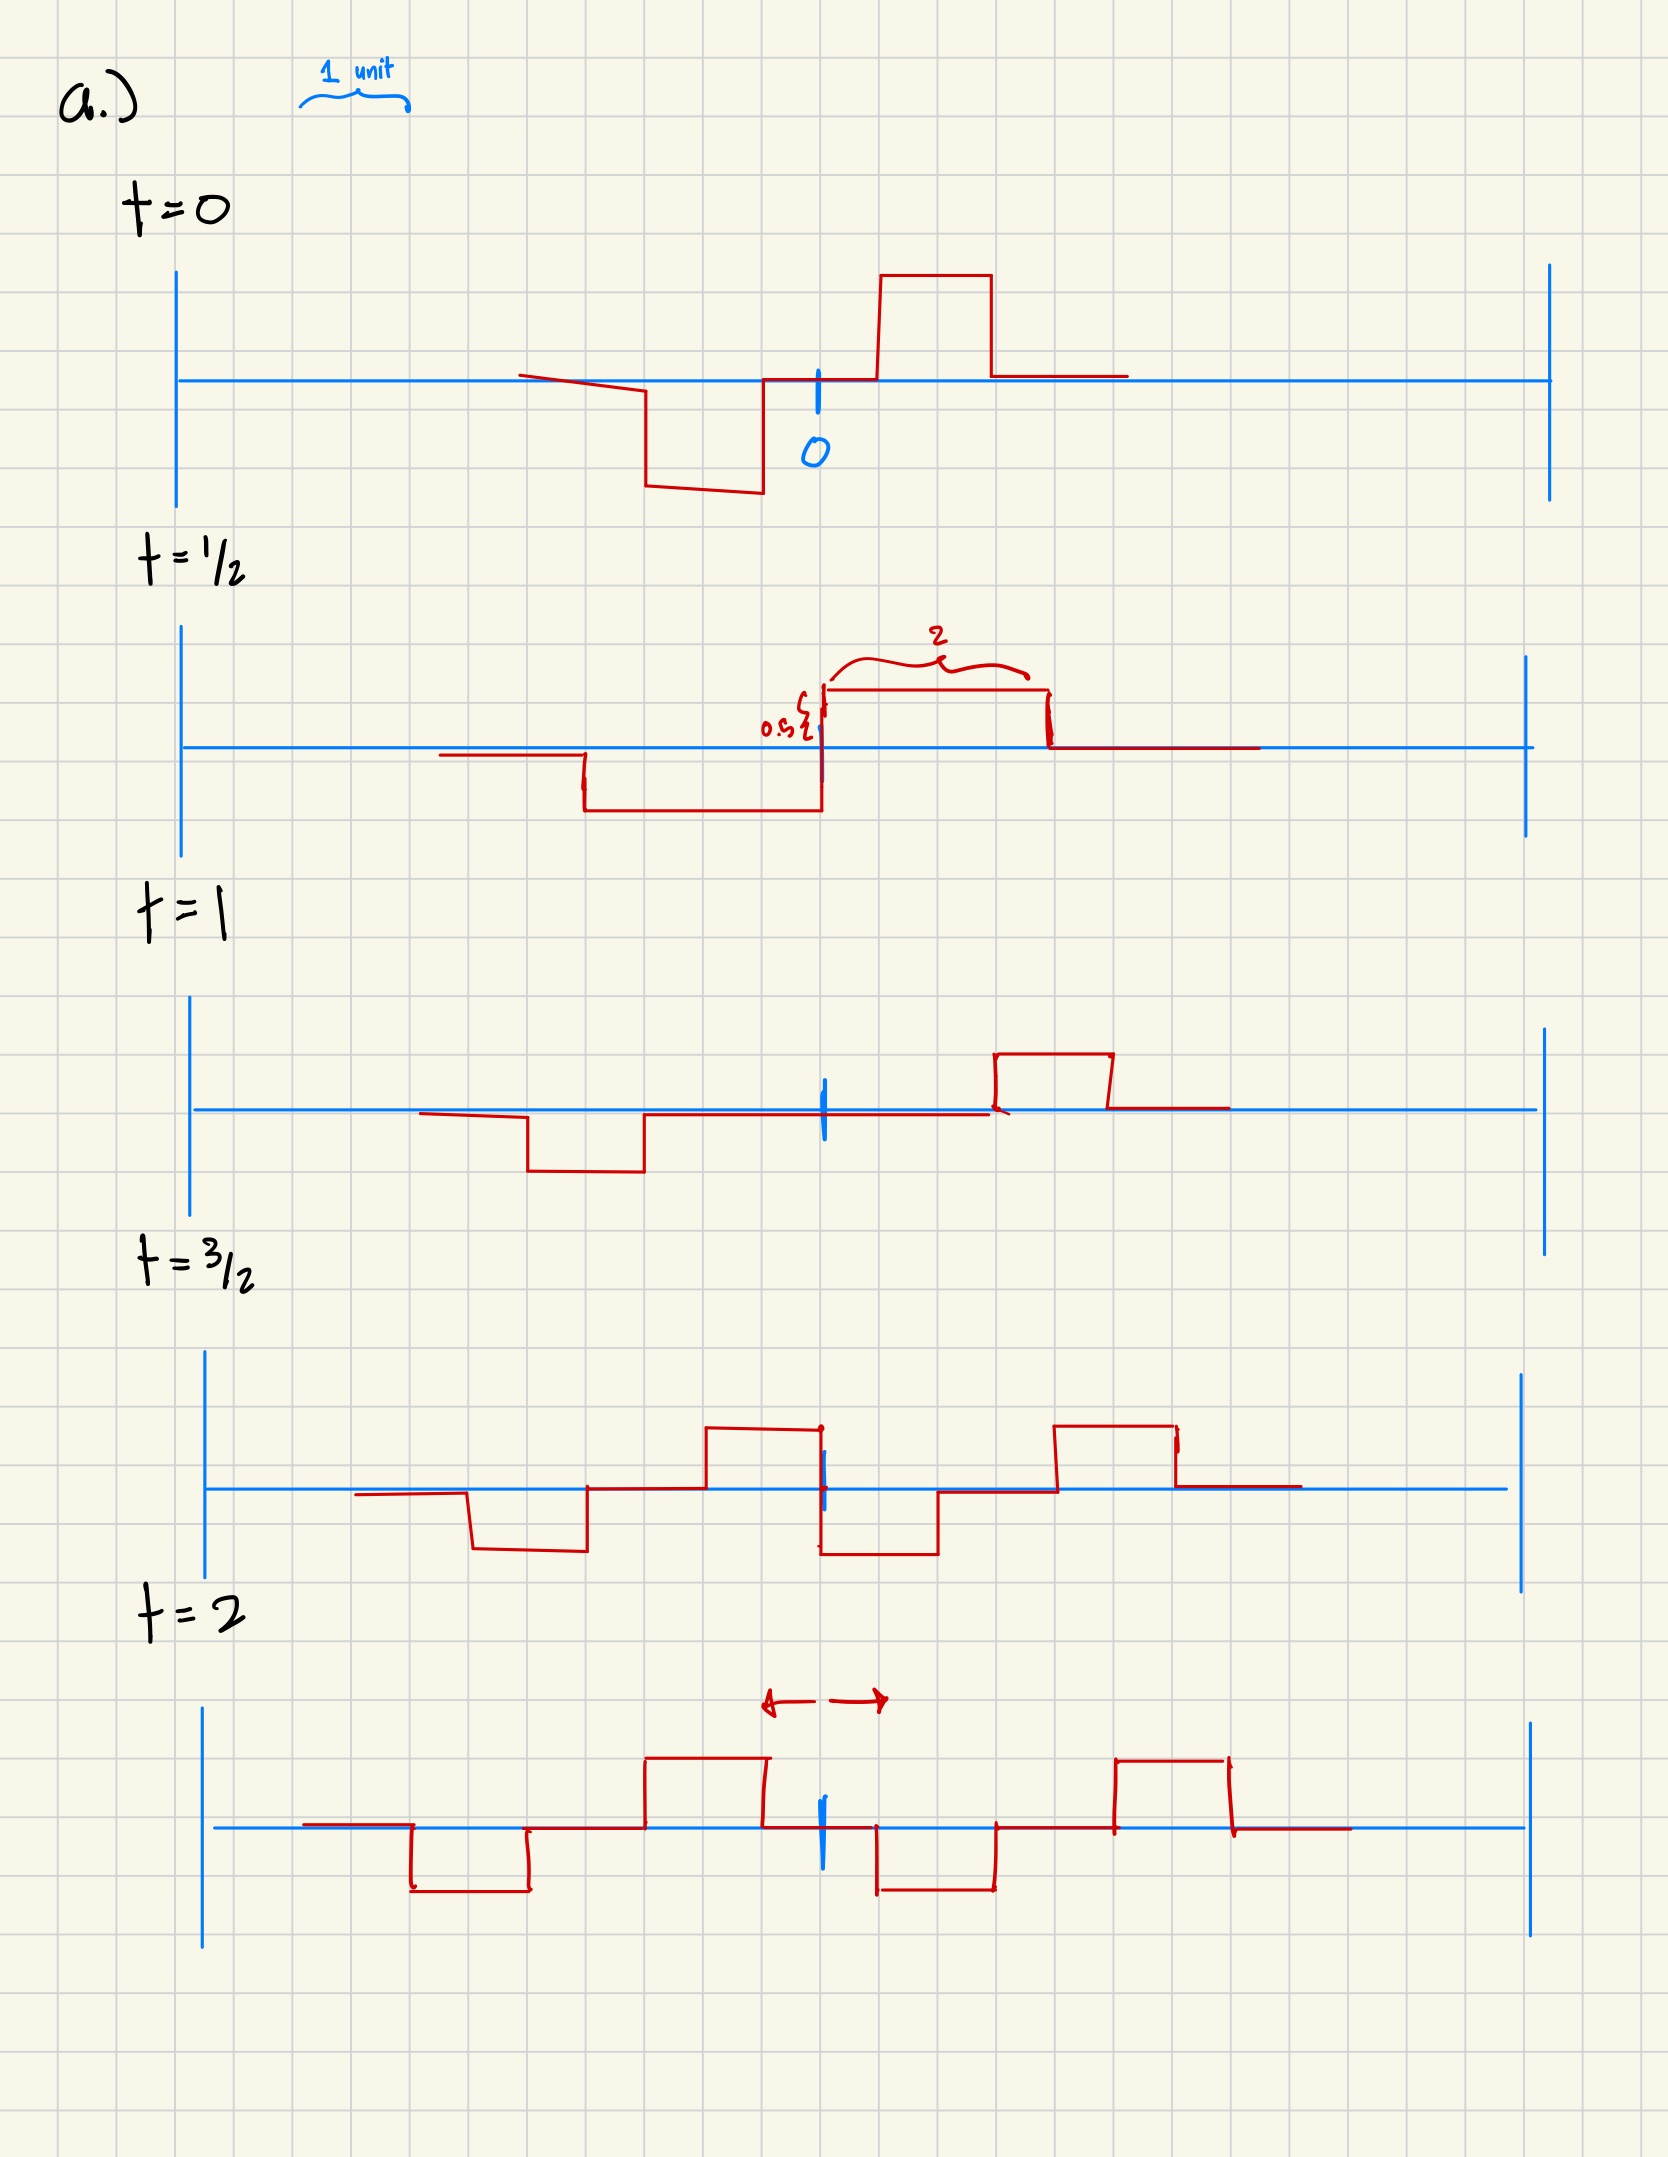
\includegraphics[width=0.4\textwidth]{HW_4_Plots-b.jpg}
    \caption{Sketch for Problem 3b. Note: 4 squares/unit}
    \label{fig:sample}
\end{figure}
\begin{figure}
    \centering
    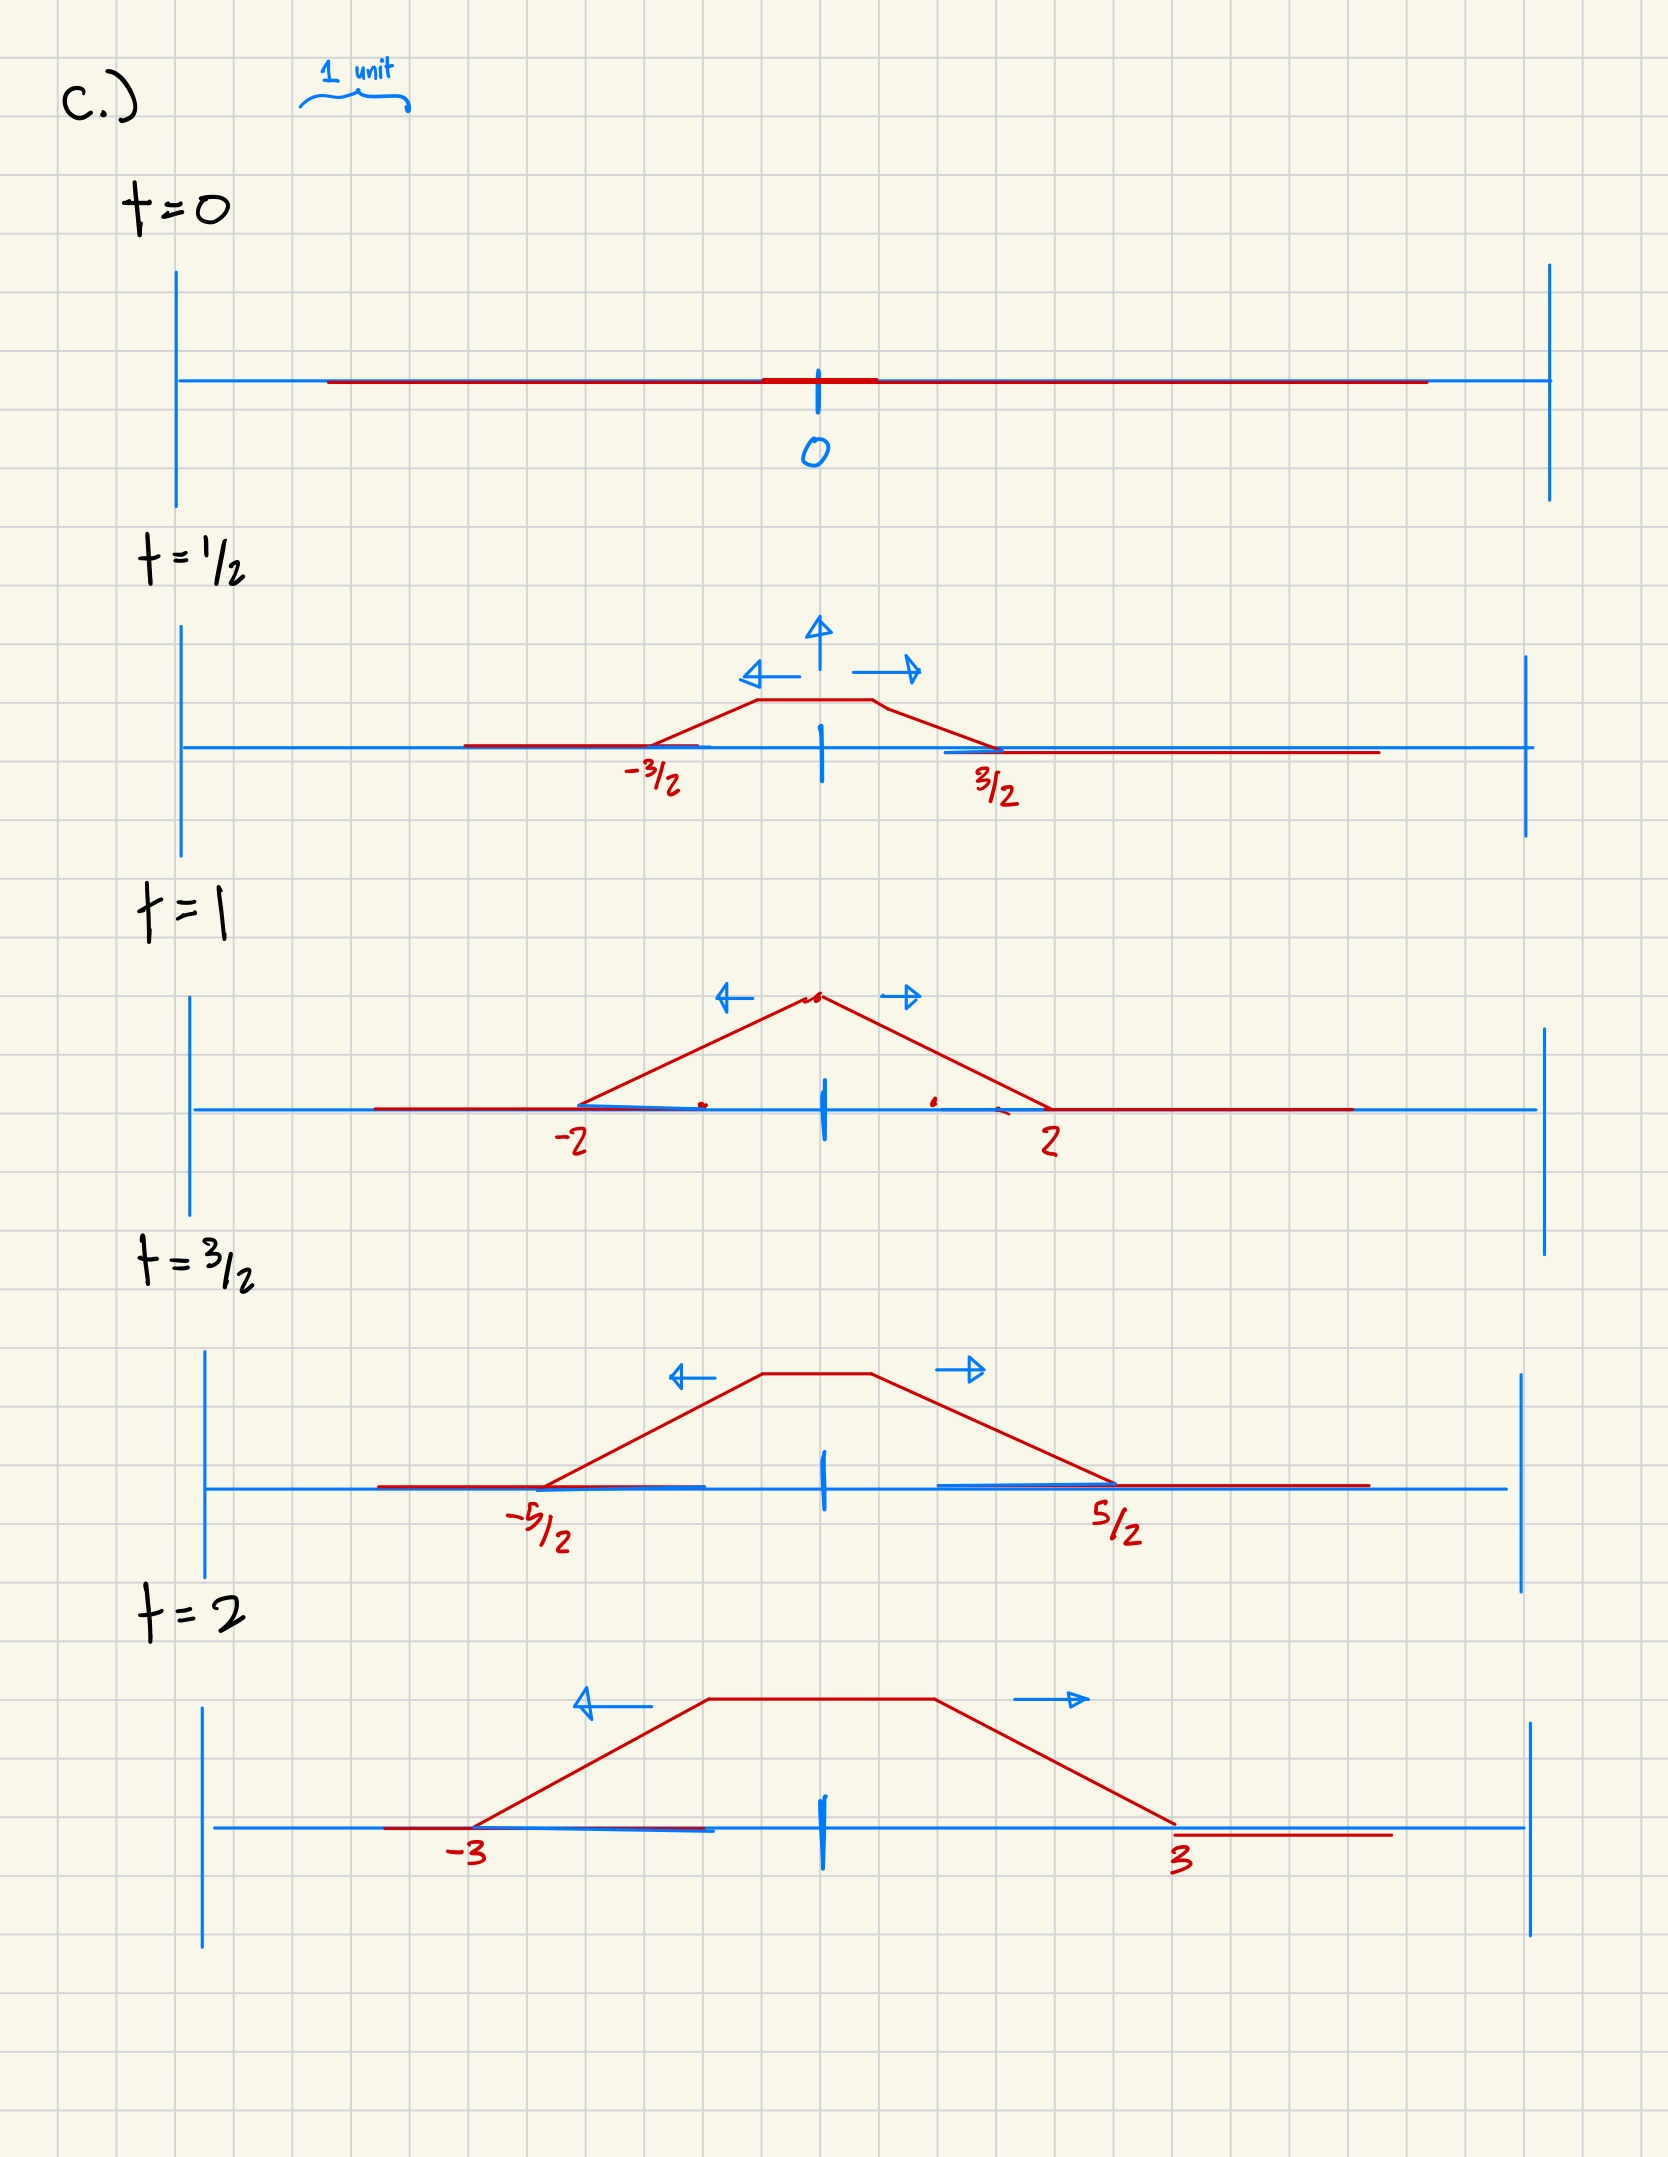
\includegraphics[width=0.4\textwidth]{HW_4_Plots-c.jpg}
    \caption{Sketch for Problem 3c. Note: 4 squares/unit}
    \label{fig:sample}
\end{figure}
\end{document}
